\chapter{Herramienta Web. Back End}
\label{backend}

Fijándonos en el diseño preliminar de la figura \ref{fig:herramienta_web_preliminar} podemos ver que nuestra aplicación Web está dividida en
\emph{front-end} y \emph{back-end}. Esta separación entre módulos es una técnica popular en diseño software. El \emph{front-end} es el encargado de
la capa de presentación, sobre este hablaremos más en el próximo capítulo. En este capítulo nos centraremos en explicar el \emph{back-end}. Este es el
encargado de procesar las peticiones provenientes del \emph{front-end} y devolver le a este la información solicitada. 
\par
El \emph{back-end} es implementado en PHP\cite{PHP}. Este es un lenguaje diseñado para desarrollo Web y además es una elección muy popular. 
Hemos utilizado ZendFramework\cite{ZF}, este es un framework orientado al desarrollo de aplicaciones Web. Junto al framework hemos utilizado
Apigility\cite{Apigility}, herramienta que simplifica la creación y mantenimiento de APIs.
\par
El \emph{back-end} tiene un enfoque RPC (llama de procedimiento remoto). Este módulo exportara un conjunto de procedimientos que pueden ser invocados
por el \emph{front-end}. Estos procedimientos realizan tareas específicas sobre un recurso concreto. A la largo de este trabajo nos referiremos
a estos procedimientos como \emph{servicios RPC}.
\par
Un aspecto oportuno destacar es que los servicios RPC son sin estado. Esto quiere decir que la respuesta a un procedimiento no es influenciada por
eventos anteriores, esta tan solo depende de los parámetros proporcionados.
\par
Si nos volvemos a fijar en la figura \ref{fig:herramienta_web_preliminar} podemos ver que en el \emph{back-end} existe la separación entre 
\emph{Modelo} y \emph{Controlador}. Esta separación sigue el patrón de diseño MVC\cite{MVCWiki}. Podemos ver que el componente de \emph{Vista} no
existe, en este caso el \emph{front-end} es nuestro componente de \emph{Vista}. Todos los servicios RPC tienen su parte proporcional de
\emph{Modelo} y \emph{Controlador}. La parte de \emph{Modelo} es la encargada de gestionar la información contenida en la base de datos. La parte de
\emph{Controllador} la encargada de gestionar los mensajes de petición y respuesta.
\par
En este capítulo procederemos a explicar los servicios RPC, pero primero explicaremos algunos aspectos técnicos como la base de datos o el ZendFramework.
\section{Protocolo de comunicación}
	Hemos explicado que entre el \emph{back-end} y \emph{front-end} existe una comunicación, para la que hemos elegido un enfoque RPC. En este
	apartado nos centraremos en un aspecto más técnico de esta comunicación. 
	\par
	Siendo la aplicación que desarrollamos una aplicación Web es de esperar que el protocolo utilizado para la comunicación entre los dos módulos
	sea \emph{HTTP}. En este protocolo se puede diferenciar entre dos tipos de mensajes, mensajes de petición y de respuesta. En nuestra
	aplicación el \emph{front-end} enviara mensajes de petición al \emph{back-end}. Los mensajes de petición especifican un campo URL, este campo
	es muy importante porque especifica el servicio RPC que se desea invocar. A la URL también son anexados los parámetros necesarios para el
	procedimiento especificado. Los mensajes de respuesta serán discutidos en el capítulo dedicado el \emph{front-end}.
\section{ZendFramework y Apigility}
	Para la realización de este trabajo hemos utilizado ZendFramework, este es un framework orientado al desarrollo de aplicaciones y servicios Web.
	Basado en PHP 5.3+ el framework sigue un diseño orientado a objetos. Esta enfocado para crear aplicaciones siguiendo el patrón MVC. Ofrece
	abstracciones para las bases de datos, autenticación y validación de parámetros. El framework también disfruta de una amplia comunidad de 
	usuarios. Todas estas ventajas nombradas anteriormente son la razón para elegir este framework en nuestro trabajo.
	\par
 	Para  los principiantes el framework ofrece la aplicación esqueleto. Esta aplicación consiste del código mínimo necesario para construir una
	aplicación usando ZendFramework, no tiene ninguna funcionalidad y esta pensada para ser extendida. En este trabajo hemos empezado con esta
	aplicación esqueleto.
  	\par
	Apigility es una herramienta creada por el equipo responsable de ZendFramework. La herramienta puede utilizarse sin necesidad del framework,
	sin embargo esta se integra muy bien con este. La herramienta facilita la creación y mantenimiento de aplicaciones Web. En nuestro caso la
	herramienta nos ha ayudado a crear los servicios RPC de nuestra aplicación. La aplicación ofrece un entorno gráfico accesible desde un navegador
	Web. El uso de la aplicación es muy fácil e intuitivo.
\section{Bases de datos}
	Tal y como hemos explicado al principio del capítulo la función del \emph{back-end} es  procesar las peticiones del \emph{front-end} y
	responderle con la información solicitada. Esta información es guardada en dos bases de datos. Para la gestión de las bases de datos
	utilizamos MySql\cite{MySql}. ZendFramework ofrece abstracciones para las bases de datos, esto facilita el trabajo con estas. En la
	figura \ref{fig:tablas} podemos ver el esquema de las tablas con las que vamos a trabajar.
	\par
	En la tabla \texttt{binTable} guardamos la información de las cuentas de cada canal. Junto a esa información guardamos las lecturas del
	barómetro, las fuentes de alta tensión y la fecha y hora actuales. La resolución de los datos es de un minuto.
	\par
	En la tabla \texttt{CALM\_ori} guardamos el valor global y  las correcciones sobre este. La lectura de presión atmosférica también es guardada.
	La resolución de estos datos es también de un minuto.
	\par
	En la tabla \texttt{CALM\_rev} guardamos la revisión de los datos de \texttt{CALM\_ori}. Vemos que la tabla tiene el mismo esquema con dos
	campos adicionales. En estos dos campos se guardan la fecha de última modificación y la versión. Los datos en esta tabla son introducidos por
	un operario. Cuando este encuentra un dato corrupto en los datos originales, puede crear una entrada en esta base de datos para señalarlo.
	\begin{figure}[h]
		\centering
		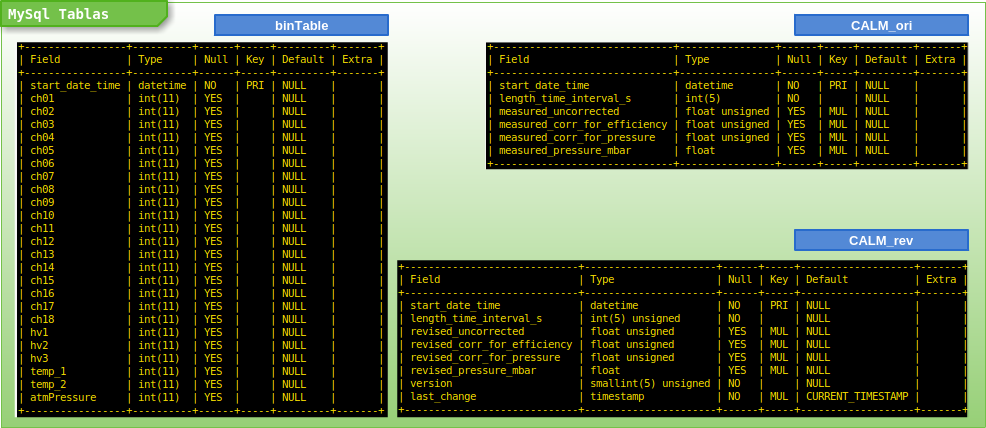
\includegraphics[keepaspectratio, width=1\textwidth]{./img/tablas.png}
		\caption{Esquema de las tablas.}
		\label{fig:tablas}
	\end{figure}
\section{Servicios REST}

